
\documentclass[a4paper,12pt, listof=totoc,toc=sectionentrywithdots]{scrartcl}

\usepackage{graphicx}

\usepackage{color}
\usepackage{listings}
\definecolor{GrayCodeBlock}{RGB}{241,241,241}
\definecolor{BlackText}{RGB}{110,107,94}
\definecolor{RedTypename}{RGB}{182,86,17}
\definecolor{GreenString}{RGB}{96,172,57}
\definecolor{PurpleKeyword}{RGB}{184,84,212}
\definecolor{GrayComment}{RGB}{170,170,170}
\definecolor{GoldDocumentation}{RGB}{180,165,45}



\usepackage{blindtext}
\usepackage{wrapfig}
\usepackage{ulem}
\usepackage[nottoc]{tocbibind}
\usepackage{setspace}

\usepackage{titling}
\renewcommand\maketitlehooka{\null\mbox{}\vfill}
\renewcommand\maketitlehookd{\vfill\null}


\title{Colorization of Grey Images by applying a Convolutional Autoencoder on the Jetson Nano}
\date{}
\author{Tim Niklas Witte and Dennis Konkol}


\lstset{
numbersep=8pt, 
frame = single, 
framexleftmargin=15pt,
framesep=1.5pt, framerule=1.5pt}

\begin{document}

\begin{titlingpage}
\maketitle
\end{titlingpage}



\tableofcontents

\pagenumbering{gobble}


\cleardoublepage
\pagenumbering{arabic}

\section{Introduction}
Embedded GPUs such as the Jetson Nano provide limited hardware resources than desktop/server GPUs.
For example, the Jetson Nano has 128 CUDA cores and 4 GB of video memory, compared to the NVIDIA GeForce RTX 3070 Ti which has 6144 CUDA cores and 8 GB of video memory.
Inference done by massive artificial neural networks (ANN) e.g. over 25.000.000 parameters on the Jetson Nano, becomes slow - about 0.01 forward pass per second.
An NVIDIA GeForce RTX 3070 Ti does 32 forward passes through the same huge ANN, and this can be achieved within a second.
This paper presents a convolutional autoencoder for grey image colorization with 300.000 parameters optimized to run on embedded GPUs.
In order to demonstrate the results during runtime on the Jetson Nano, the live grey camera stream is colorized, as shown in Figure~\ref{fig:OpenCV_window}.  

\begin{figure}[h]
\centering
        \includegraphics[totalheight=4cm]{Figures/OpenCV_window.png}
    \caption{OpenCV window on the Jetson Nano displaying the original, grey, colorized camera stream and corresponding loss between original and colorized image.}
    \label{fig:OpenCV_window}
\end{figure}

This paper is organized as follows:
The concept of a convolutional autoencoder will be covered in section 2.
Section 3 explains the necessary software and hardware setup on the Jetson Nano.
The training procedure, including the model architecture, is discussed in section 4.
Optimization techniques of our model considering running on the Jetson Nano are presented in section 5.
In section 6, the performance of our model is evaluated by comparing the colorized images generated by our models and by a state-of-the-art ANN for grey image colorization, which has about 25.000.000 parameters.
Finally, the final results are summed up in section 7.

\section{Convolutional Autoencoder}

\subsection{Convolutions}

Convolutions detect features and extract these from images by applying a filter kernel which is a weight matrix.
As shown in Figure ~\ref{fig:convolution}, a convolution iterates a filter kernel over the entire image.
During each iteration, an area with the same size as the kernel is processed by an element-wise multiplication followed by summing each value up, representing the result for the area of this image.
This area is shifted one step (depending on side size) further to the right in the next step. 
The same processing step occurs again.

\begin{figure}[h]
\centering
        \includegraphics[totalheight=5cm]{Figures/convolution.png}
    \caption{Concept of a convolution~\cite{ConvolutionAnimation}.}
    \label{fig:convolution}
\end{figure}


\subsection{Autoencoder}

Autoencoders are artificial neural networks used to learn features of unlabeled data.
As presented in Figure~\ref{fig:autoencoder}, the encoder part compresses the data by gradually decrease of the layer size.
The resulting embedding/code is passed to the decoder part responsible for
reconstructing it.
In the decoder, the layer size increases per layer.
Overall, the input \texttt{X} and output \texttt{X'} shall be the same.

\begin{figure}[h]
\centering
        \includegraphics[totalheight=5cm]{Figures/Autoencoder.png}
    \caption{An Autoencoder compresses and decompresses the data~\cite{autoencoderImg}.}
    \label{fig:autoencoder}
\end{figure}

Instead of fully connected layers, a convolutional autoencoder applies convolutions in the encoder and transposes convolutions in the decoder.

\section{Setup}

\subsection{Software}
TensorFlow was installed following the official guide from NVIDIA~\cite{jetsonNanoTensorFlow}.
Furthermore, it is not recommended to install the current version of OpenCV via pip3 due to compatibility issues with the CSI camera.
The CSI camera i.e. the \texttt{gstream} can only be accessed with an OpenCV version lower than 3.3.1.
This version was installed manually by downloading the source code from the official website and compiling it~\cite{opencv}.
Besides, for speed purposes, the maximal performance mode was enabled by the command \texttt{sudo nvpmodel -m 0}.
In order to enable the Jetson Clock, the command \texttt{sudo jetson\_clocks} was used.


\subsection{Hardware}
The CSI camera was plugged into the corresponding slot in the Jetson Nano.
Furthermore, the HDMI display shows the OpenCV window as presented in Figure~\ref{fig:OpenCV_window}.


\section{Training}

\begin{wrapfigure}{r}{.4\textwidth}

\centering
        \includegraphics[totalheight=6cm]{Figures/LossPlot.png}
    \caption{Train and test loss during training.}
    \label{fig:trainTestLoss}

\end{wrapfigure}
At the beginning of training our model, we used the common RGB color space.
In other words, the input was the grey scaled image, and the output was the RGB image.
However, we lost too much information in the picture.
So the general input picture was detectable but with a lot of "compression".
The reason for this is that for one pixel, all three values of RGB are responsible for the brightness of that pixel.
So it is possible to get the right color but not the correct brightness. That is why we switched to the CIE LAB color space.
Here we also have three values for each pixel, the L channel for the
'brightness' and A and B as the color channel.
The L channel is like the grayscale image for the model.
The model's output is two values, the A and B channels.
So with the combination of the given A, B, and our old L values, we get the colored image. We get an overall correct image because of the kept L channel, even if the colors would not match the original
image.

The model was trained for 13 epochs (in total: 15 hours) with the ImageNet2012 dataset.
It contains ca. 1.300.000 training images and 300.000 validation images used for test data.
As presented in Figure~\ref{fig:trainTestLoss} the model was successfully trained to convergence because, after about ten epochs, the train loss does not change significantly ($< 0.0001$) compared with the loss to the next epoch.


\subsection{Model}
As shown in Listing~\ref{lst:ourModel_summary}, our convolutional autoencoder has about 300.000 parameters.
The model's memory size is about 1.2 MB ($300000 \cdot 4$ Byte).
Encoder and decoder parts of the ANN are equally balanced due to having almost the same amount of parameters.

\begin{lstlisting}[language=bash, caption=Parameter amount of our model (output of \texttt{summary()} call)., label={lst:ourModel_summary}, basicstyle=\fontsize{11}{9}\selectfont\ttfamily]
 Model: "autoencoder"
_______________________________________________________________
 Layer (type)                Output Shape            Param #   
===============================================================
 encoder (Encoder)           multiple                148155    
                                                               
 decoder (Decoder)           multiple                150145    
                                                                 
===============================================================
Total params: 298,302
Trainable params: 297,210
Non-trainable params: 1,092
_______________________________________________________________
\end{lstlisting}


Figure~\ref{fig:EncoderLayer} and~\ref{fig:DecoderLayer} present the structure of the layers contained in the encoder and decoder.
The encoder receives a 256x256 pixel grey image.
Due to the grey color, there is only one color channel.
Convolutions can be seen as feature extractors.
At the first convolution in the encoder (see \texttt{Conv2D\_0} in Figure~\ref{fig:EncoderLayer}), there are 75 features extracted from this grey image.
These extracted features are represented as channels (similar to color channels but not colors) called feature maps.
Literally speaking, a feature map could be seen as a heatmap in which the pixel belonging to the corresponding feature has a high magnitude.
Due to the stride size of 2, the size of these features maps is halved.
A convolution operation is followed by a batch normalization layer and an activation layer (the drive is normalized before its goes into the activation function).
In the encoder this occurs four times.
With each step, the amount of filters increases.

\begin{figure}[h]
  \centering
  \begin{minipage}[b]{0.4\textwidth}
    \includegraphics[width=\textwidth]{Figures/EncoderLayer.png}
    \caption{Encoder layers.}
    \label{fig:EncoderLayer}
  \end{minipage}
  \hfill
  \begin{minipage}[b]{0.4\textwidth}
    \includegraphics[width=\textwidth]{Figures/DecoderLayer.png}
    \caption{Decoder layers.}
    \label{fig:DecoderLayer}
  \end{minipage}
\end{figure}


The resulting embedding is passed into the decoder.
Instead of convolutions reducing the feature map size, transpose convolutions increase the feature map size by a factor of 2.
Like the encoder, a transpose convolution is followed by batch normalization and activation layers.
In the decoder this occurs four times.
With each step, the amount of filters decreases.
Except for the last transpose convolution, which is a bottleneck layer:
It decreases the amount of filters from 75 to 2 (\textit{a} and \textit{b} channel) and keeps the feature map size constant (stride size = 1).


\section{Optimizing the model to run on the Jetson Nano }


\begin{wrapfigure}{r}{.4\textwidth}

\centering
        \includegraphics[totalheight=4cm]{Figures/ResidualConnection.png}
    \caption{Concept of a residual connection~\cite{residualConnectionImg}.}
    \label{fig:ResidualConnection}

\end{wrapfigure}

Residual connections also called skip connections in neural networks, face the vanishing gradient problem (tiny weight adjustments~\cite{vanishingGradients}) in the backpropagation algorithm~\cite{resnet}.
As shown in Figure~\ref{fig:ResidualConnection}, the output \texttt{x} of a layer is added two layers further to the input of the third layer~\cite{resnet}.
The output \texttt{x} must be saved due to it is used in a later time step.
Therefore, residual connections need a lot of GPU memory, causing a outsource of a part of other data needed for the model.
To speed up the FPS, our model does not have residual connections.

As mentioned in the first section, the Jetson~Nano has 128 CUDA cores.
The amount of filters per layer does not exceed this number of cores.
This limitation enables TensorFlow simple scheduling of a feature map calculation to a specific core during the output calculation of a layer.
In other words, there are no cores that must do a second filter map calculation after the first one while other cores are idling.
The calculation of a previous layer must be finished before starting with the next layer.
Furthermore, limiting the amount of filer reduces the model size.

In Deep Learning, overparameterization often occurs:
As a result, the number of trainable parameters is much larger than the number of training examples.
As a consequence, the model tends to overfit the data~\cite{overparameterization}.
The opposite applies to our model.
Literally speaking, our model is "under-parameterized" -
Due to there being only 300.000 parameters on about 1.3 million training images, our model is forced to generalize as strong as possible during training.
To archive such generalization the model is trained multiple epochs (iteration over the entire training dataset).
It is assumed that such generalization results in similar results compared with a model which has considerable amounts of parameters.
In other words, the higher costs for training a small model compared with a larger model shall result in similar results but the latency to generate the result with the smaller model is lower.
Besides, the non-existence of skip connections increases the chance of vanishing gradients during training.
Although, multiple training epochs compensate this problem.
To clarify, millions of tiny weight changes sum up into an effective weight adjustment.


\section{Evaluation: Compare with Colorful Image Colorization}

As demonstrated in Listing~\ref{lst:theirModel_summary}, the Colorful Image Colorization model from Richard Zhang et al. has about 25 million parameters~\cite{colorize}.
The model presented in this paper is about 80 times smaller. 
Its input shape is 256x256x1 and the same as our model.

\begin{lstlisting}[language=bash, caption=Parameter amount of the Colorful Image Colorization model (output of \texttt{summary()} call)., label={lst:theirModel_summary}, basicstyle=\fontsize{11}{9}\selectfont\ttfamily]
Model: "ColorfulImageColorization"
_______________________________________________________________
 Layer (type)                Output Shape              Param #   
===============================================================
[...]   
                                                                 
===============================================================
Total params: 24,793,081
Trainable params: 24,788,345
Non-trainable params: 4,736
_______________________________________________________________
\end{lstlisting}


Figure~\ref{fig:ColoredImages_compareModels} shows grey images colorized by the Colorful Image Colorization model~\cite{colorize} and by our model. 
Our model tends to colorize the images with a grey touch and the colors are not saturated compared with the Colorful Image Colorization model.



\begin{figure}
\centering
        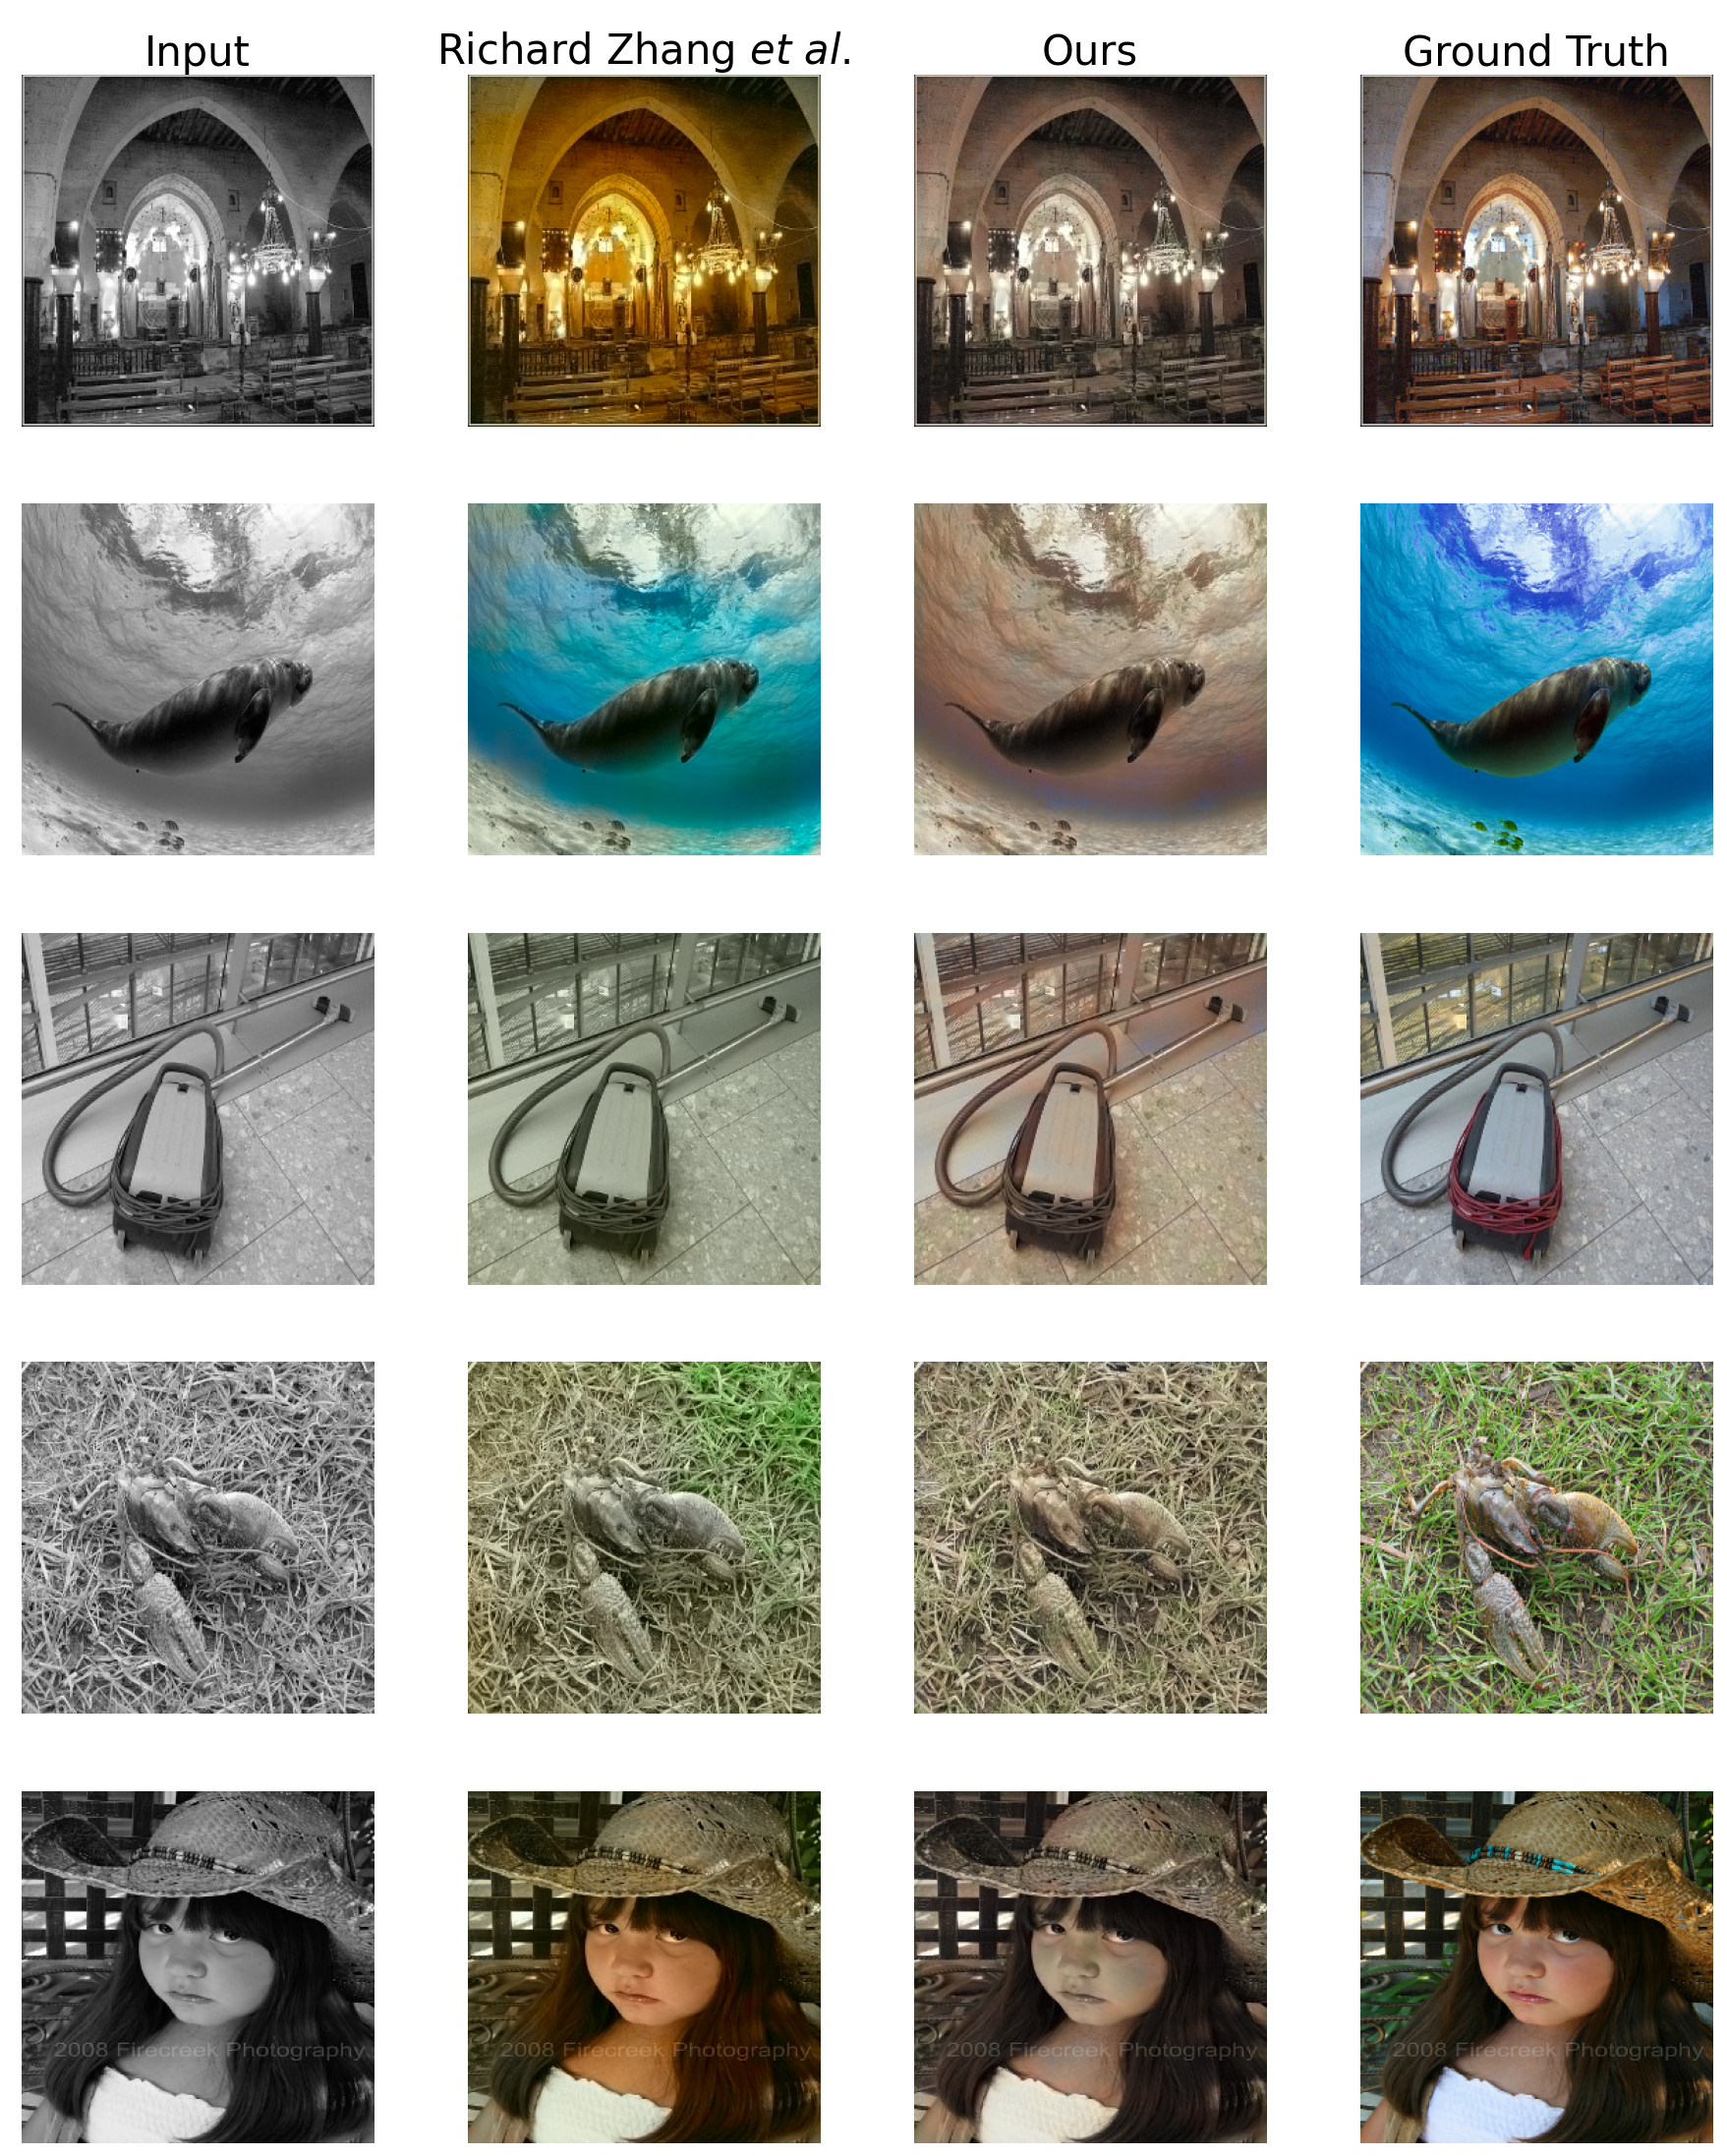
\includegraphics[totalheight=13cm]{Figures/ColoredImages_compareModels.png}
    \caption{Colorized images generated by the Colorful Image Colorization model from Richard Zhang et al. and by our model.}
    \label{fig:ColoredImages_compareModels}
\end{figure}


Our model does regression by predicting the \textit{ab} values.
The model output shape is 256x256x2 (see \texttt{tanh\_3} in Figure~\ref{fig:DecoderLayer}).
In contrast to the model from Richard Zhang et al., classification is applied here:
There is a probability distribution for each pixel approximating which color it may be.
For demonstration purposes, there were 313 colors available.
As a consequence, the model output shape is 256x256x313~\cite{colorize}.
Compared to our model, the larger output shape requires a more extensive (ca. 80 times) amount of parameters.



\begin{figure}[h]
\centering
        \includegraphics[totalheight=6cm]{Figures/ColorizedImagesLossPlot_comparedModels.png}
    \caption{Loss based on colorized images by the 
    Colorful Image Colorization model from Richard Zhang et al. and by our model.}
    \label{fig:Loss_compareModels}
\end{figure}

Considering the loss as shown in Figure~\ref{fig:Loss_compareModels},
our model outperforms the model from Richard Zhang et al.
However, the euclidean loss (mean squared error) $L_2(\hat{y}, y)$ for the prediction $y$ and the target (also called ground truth) $\hat{y}$ was applied:

\[ L_2(\hat{y}, y) = \frac{1}{2} \cdot \sum_{h,w} || y_{h,w} - \hat{y}_{h,w} ||^{2} \]

The loss function is ambiguous for the colorization problem.
Consider the prediction $y$ for a single pixel with a loss of $d$:
There are two corresponding targets $\hat{y} = y \pm d$ possible instead of a single one.
Furthermore, consider a set of pixels. For each of these pixels, a corresponding color will be predicted.
The optimal solution is the mean of all pixels within this set.
In the case of color prediction, this averaging causes a grey bias and desaturated colors~\cite{colorize}.



\section{Conclusion}


Our model predicts the most possible color by applying regression.
In contrast to the model proposed by Richard Zhang et al. which classifies the most possible color.
Due to the one-hot encoding applied for these color classifications, over 80 times more parameters are needed as required for our model, considering the parameter balance between hidden layers and output layers.
Comparing the colorized images generated by an ANN based on classification and by regression, regression-based ANN tends to colorize images with a grey touch and unsaturated colors because of an ambiguous loss function for the colorization problem.
However, the results are acceptable considering the difference in the number of parameters between the two models.
Furthermore, a GPU cannot ultimately accelerate a classification-based model because the last part of the model is a sampling process.
This process is an argmax operation over 313 possible colors (see model shape) which runs on the CPU.
Note that transferring data from GPU to CPU could be seen as a performance bottleneck.

Overall, our model archives about 10 FPS on the Jetson Nanos.
Running the Richard Zhang et al. model will result in less than 0.01 FPS.



 






\bibliographystyle{ieeetr}
\bibliography{Literatur}

\end{document}

